\chapter{Introduction}

\iffalse

-  Illustrative Example Scenarios
-  Technical Challenges
-  Core Contributions
-  Other Contributions
-  What isnt the thesis dealing with?

\fi
\begin{itemize}
    \item  Exploiting deep learning, we can extract various types of information from a data distribution.
    \item Extracting relevant information is useful in a large number of contexts such as story generation, targeted captioning, etc. 
    \item Representation Learning thus far has been defined in the context of deep learning techniques but not grounded in NLP. 
    \item De-Entanglement is a framework aimed at extracting relevant information by systematically isolating the factors of variation. 
    \item Factors could be user defined - from attributes such as color, accent all the way upto schema or recipe stages.
    \item This thesis is concerned with developing tools to solve this 
    \item Having developed these tools, show  that can be useful for a downstream task as well. VQA, Audio search.

    
\end{itemize}

\begin{itemize}
    \item \textbf{What is missing in the current literature} : No consensus as to which is better and why. Is there a universal? Depending upon a task of choice, is there a specific one to use? Why?
    
    \item \textbf{Core Contribution}: Attempt to move towards a taxonomy grounded in NLP, so that we can start discussion towards categorization of the approaches. 
    
    \item Literature motivates the development of a method with the generality of A=self supervised approaches while incorporating prior information, like the latter. prior works have been developed largely independently without grounding in NLP. If we hope to push research and understanding of these methods forward, it is desirable to have a set of common lingua(guiding principles) and concrete, yet sufficiently general problem statement. I hope to work towards such guidelines in this thesis. ( Nature vs nurture, even humans cannot do). 
    
    
\end{itemize}

\section{Motivation}

\textbf{Ability to extract useful information is important} \\

Often we are faced with scenarios where we need to extract relevant information from the distribution of data. Let me elucidate this specifically in the context of generative models. There are several categories of generative models and each category has a different information requisites. In all the categories, it is essential to have explicit control over the process of content generation. 

\begin{itemize}
    \item For example, consider speech to speech translation. It is a scenario where the input and output are comparable in terms of length of content. However, We might need to focus on a particular word depending on context. Consider translating the sentence `John loves Mary' into a different language. Depending on the context, the system has to be able to emphasize one of the words (It is John who is loving Mary - JOHN loves Mary vs Mary is the one being loved by John - John loves MARY).
    
    \item Imagine having to deliver content through voice media such as Alexa or Siri. It would be nice to be able to summarize content and tell what is relevant instead of blurting out everything. Other examples include text summarization for headline generation. 
    
    \item In other cases, we need to expand. Simplest example for this is Text to Speech Synthesis. For other examples, consider any task that involves conversion of structured data such as table to unstructured such as free form text or speech. In such cases, it is useful to have a representation that embeds some sort of `structure' of long form content of interest so that we can target the generative model to closely follow this structure. Examples include newspaper article generation. 
    
    \item   Imagine going on a space ship and the robot telling you everything is doomed. In such cases, we need to convey the content but use a speaking style that is calming and soothing. Consider speech enhancement or source separation as example tasks.

\end{itemize} 

\begin{figure}[t]
\centering
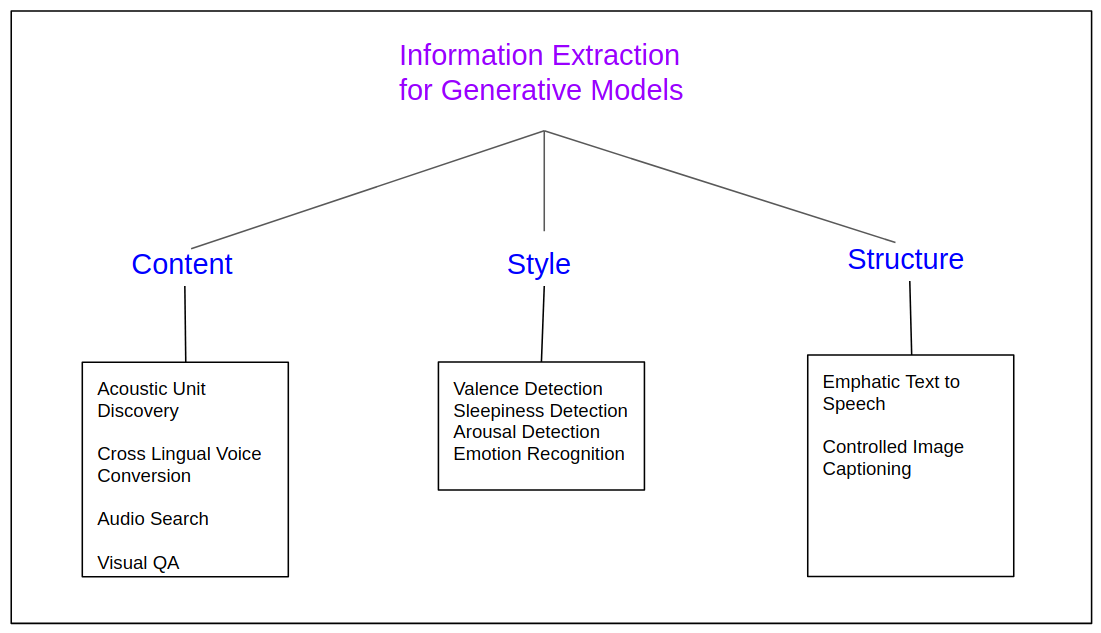
\includegraphics[scale=0.4]{LatexDiss/Dissertation/images/taxonomy.png}
\caption{\textit{A Basic Taxonomy depicting different components for information extraction}} 
\label{taxonomy}
\end{figure}  

%  This includes applications such as text summarization for headlines, long form  content generation for article generation, etc. In such scenarios, i

\textbf{Challenges for controlled generation} 

\begin{itemize}
    \item Sparsity: The control factors are under specified 
    
\end{itemize}
\subsection{De-Entanglement}
Imagine a property of a model of the world referred to as De-Entanglement. It is (currently) defined as the ability to isolate the factors of variation which perhaps were involved in the design of the world itself. It is easy to see that such a property is extremely desirable in a model. Consider kids playing with Lego toys as opposed to a static toy like a TeddyBear or a Barbie. The freedom to dismantle the structure apart and re-compose variants of it has been shown to improve creativity \cite{gauntlett2014lego}. The implications become even more apparent when we consider a real life application such as speech processing. It is extremely difficult to reason about speech in the time domain by inspecting the individual samples. However, transforming the same utterance into frequency domain by applying Fourier Transform - a process that isolates the contribution from individual frequencies - makes reasoning easier, to the point of even identification of the individual linguistic units within the utterance. In this context, the individual frequencies and their contributions are the factors of variation in the generative process of speech data. The observation can be extended to other types of data as well. Consider spectroscopy: The ability to spectrally decompose (visible) light enables estimation of cosmic evolution of celestial bodies \cite{stellar_evolution}. The argument presented above claims that such isolation should invariably help downstream tasks. However, this does not appear to be always true. Consider as example the task of adding two natural numbers. Perhaps an appropriate de-entanglement for a model aimed at completing this task involves Peano axioms \cite{peano_axioms}. But we as humans have been conditioned to solve this task by cumulative addition of individual digits with appropriate carryover and not necessarily following \cite{peano_axioms}. Similarly consider  the inner workings of AlphaZero \cite{alpha_zero_withouthumans}. It is not clear if the self learning based algorithm is accomplishing an isolation of relevant factors of variation in the latent space. Moreover, there are scenarios where estimation of causal factors is intractable. In such scenarios, it appears hard to comment about performance with respect to a concept like de-entanglement. 

Within the scope of my work, I am interested in investigating the extent to which  isolation of factors of variation as mentioned above is plausible and useful in the context of Natural Language Processing(NLP). In this context, `De-Entanglement' refers to the ability of a model to isolate the relevant causal factors of variation in the joint distribution spanned by the input and output distributions defined by the task at hand. Specifically, I am interested in answering some of the following research questions:
\begin{itemize}
    \item What are the scenarios where de-entanglement helps solve the task?
    \item In cases where true, does de-entanglement help solve the task more efficiently? How is efficiency manifested? In making the model more compact? Making the algorithm faster?
    \item In cases where true and de-entanglement does not result in a more efficient solution, why does this happen? 
    \item What are the scenarios where de-entanglement cannot help solve the problem? Is it due to probabilities becoming too miniscule? Is it because the calculations seem implausible given the current compute? 
    \item In cases where de-entanglement cannot be applied but seems reasonable, can we reformulate the problem or task so that we can apply de-entanglement? 
    \item Are there cases where de-entanglement hurts the model? Does it do so by limiting the expressivity of models? Are there any model blindsplots in these scenarios? 
    \item Why is de-entanglement preferable? Is it since it avoids adversarial attacks?
    \item What are some of the challenges for de-entanglement? What is difficult about it? sparsity? lack of ability to identify the factors of variation? example: sentiment analysis
    \item What are the approaches to accomplish de-entanglement? 
    
\end{itemize}



\section{Organization of Thesis}

In this thesis, I propose to extract the following types of information from the distribution of data:

\begin{itemize}
    \item Content. In this thesis, I specifically focus on acoustic phonetic content. I show examples from Acoustic Unit Discovery and Source separation.
    \item Style. In this thesis, I focus on paralinguistic style of an utterance. I show examples from sleepiness detection, valence and arousal detection. I apply the findings to code mixed speech synthesis.
    \item Structure. I specifically concern myself with prosodic structure of an utterance. I present examples from image captioning and emphasis based text to speech. 
\end{itemize}
